


% Default mode is landscape, which is what we want, however dvips and
% a0poster do not quite do the right thing, so we end up with text in
% landscape style (wide and short) down a portrait page (narrow and
% long). Printing this onto the a0 printer chops the right hand edge.
% However, 'psnup' can save the day, reorienting the text so that the
% poster prints lengthways down an a0 portrait bounding box.
%
% 'psnup -w85cm -h119cm -f poster_from_dvips.ps poster_in_landscape.ps'

\documentclass[a0]{a0poster}
% You might find the 'draft' option to a0 poster useful if you have
% lots of graphics, because they can take some time to process and
% display. (\documentclass[a0,draft]{a0poster})

%%
%% MATH DEFINITIONS   
%%

\def\({\left(}
\def\){\right)}

\def\inv#1{{\frac{1}{#1}}}
\def\ddt#1{\der{#1}{t}}
\def\ddx#1{\der{#1}{x}}
\def\ddz#1{\der{#1}{z}}
\def\der#1#2{{\frac{d#1}{d#2}}}
\def\derder#1#2{{d^2\frac{#1}{d{#2}^2}}}
\def\norm#1{\labs #1 \rabs}
\def\pder#1#2{{\frac{\partial#1}{\partial#2}}}
\def\pderder#1#2{{\frac{\partial^2#1}{\partial{#2}^2}}}
\def\pdt#1{\pder{#1}{t}}
\def\pdx#1{\pder{#1}{x}}
\def\pdxx#1{\pderder{#1}{x}}
\def\pdz#1{\pder{#1}{z}}
\def\pdzz#1{\pderder{#1}{z}}
\def\ssize#1{{\scriptsize #1}}

\def\bmat{\left[ \begin{array}}
\def\bna{\begin{array}}
\def\bneas{\begin{eqnarray*}}
\def\bnea{\begin{eqnarray}}
\def\bnes{\begin{displaymath}}
\def\bne{\begin{equation}}

\def\emat{\end{array} \right]}
\def\ena{\end{array}}
\def\eneas{\end{eqnarray*}}
\def\enea{\end{eqnarray}}
\def\enes{\end{displaymath}}
\def\ene{\end{equation}} 

\def\half{\frac{1}{2}} 

\def\revrxn#1#2{
\begin{array}{c} 
{#1}\\
\rightleftharpoons \\
{#2}
\end{array}
}

\def\Bold#1{\vspace{0.1in} \noindent {\bf \boldmath #1}}

\def\Sec#1{Section~\ref{#1}}
\def\Secs#1#2{Sections~\ref{#1}--\ref{#2}}
\def\SecsAnd#1#2{Sections~\ref{#1} and \ref{#2}}

\def\Eqn#1{Eq.~\ref{#1}}
\def\Eqns#1#2{Eqs.~\ref{#1}--\ref{#2}}
\def\EqnsAnd#1#2{Eqs.~\ref{#1} and \ref{#2}}

\def\Eq#1{Eq.~\ref{#1}}
\def\Eqs#1#2{Eqs.~\ref{#1}--\ref{#2}}
\def\EqsAnd#1#2{Eqs.~\ref{#1} and \ref{#2}}

\def\Fig#1{Fig.~\ref{#1}}
\def\Figs#1#2{Figs.~\ref{#1}--\ref{#2}}
\def\FigsAnd#1#2{Figs.~\ref{#1} and \ref{#2}}

\def\Figure#1{Figure~\ref{#1}}
\def\Figures#1#2{Figures~\ref{#1}--\ref{#2}}
\def\FiguresAnd#1#2{Figures~\ref{#1} and \ref{#2}}

\def\avg#1{\langle{#1}\rangle}
\def\Parens#1{\left({#1}\right)}

\def\Bold#1{{\bf #1}}
\def\Block#1#2{{\bf #1:} {#2}\\ }

\def\bfcite#1{{\bf\cite{#1}}}

\def\bpi{\boldsymbol \pi}
\def\E{\mathsf E}
\def\P{\mathsf P}
\def\Pr{\mathsf P}
\def\Var{\mathsf{Var}}


%%
%% CALCIUM DEFINITIONS   
%%

% My Definitions

\def\FcepsilonR1{Fc$\epsilon$R1}

\def\Ps{$\ps$}
\def\ps{{\rm s}^{-1}}

\def\Pms{$\pms$}
\def\pms{{\rm ms}^{-1}}

\def\UM{$\uM$}
\def\uM{\mu{\rm M}}

\def\Um{$\um$}
\def\um{\mu{\rm m}}

\def\Us{$\us$}
\def\us{\mu{\rm s}}

\def\Ums{$\ums$}
\def\ums{\mu{\rm m}^2}

\def\Nm{$\nm$}
\def\nm{\mu{\rm m}}

\def\Pumps{$\pumps$}
\def\pumps{\mu{\rm M}^{-1} {\rm s}^{-1}}

\def\Pumpms{$\pumpms$}
\def\pumpms{\mu{\rm M}^{-1} {\rm ms}^{-1}}

\def\UMps{$\uMps$}
\def\uMps{\mu{\rm M}/{\rm s}}

\def\Umpss{$\umpss$}
\def\umpss{\mu{\rm m}/{\rm s}^2}

\def\Umsps{$\umsps$}
\def\umsps{\mu{\rm m}^2/{\rm s}}

\def\Umspms{$\umspms$}
\def\umspms{\mu{\rm m}^2/{\rm ms}}

\def\Ryr{RyR}
\def\ip{{[{\rm IP}_3]}}

\def\Ip{${\rm IP}_3$}
\def\Ipr{${\rm IP}_3{\rm R}$}

\def\cad{[{\rm Ca}^{\rm 2+}]_{\rm d}}
\def\Cad{$\cad$}

\def\cabulk{[{\rm Ca}^{\rm 2+}]_{\rm bulk}}
\def\Cabulk{$\cabulk$}

\def\cainf{[{\rm Ca}^{\rm 2+}]_{\infty}}
\def\Cainf{$\cainf$}

\def\cai{[{\rm Ca}^{\rm 2+}]_{\rm i}}
\def\Cai{$\cai$}

\def\caext{[{\rm Ca}^{\rm 2+}]_{\rm ext}}
\def\Caext{$\caext$}

\def\cae{[{\rm Ca}^{\rm 2+}]_{\rm ER}}
\def\Cae{$\cae$}

\def\cat{[{\rm Ca}^{\rm 2+}]_{\rm T}}
\def\Cat{$\cat$}

\def\ve{{\varepsilon}}
\def\Bj{${\rm B}_j$}
\def\B{${\rm B}$}
\def\Bt{$\bt$}
\def\Ca{${\rm Ca}^{\rm 2+}$}
\def\K{${K}^{+}$}
\def\Cabj{${\rm CaB}_j$}
\def\Cab{${\rm CaB}$}
\def\Kj{$\kj$}
\def\Kjm{$\kjm$}
\def\Kjp{$\kjp$}
\def\Kmm{$\kmm$}
\def\Kkm{$\kkm$}
\def\Kmp{$\kmp$}
\def\Km{$\km$}
\def\Kp{$\kp$}
\def\bjt{\bj_T}
\def\b{[{\rm B}]}
\def\bj{[{\rm B}_j]}
\def\bmt{\bm_T}
\def\bt{\b_{\rm T}}
\def\bm{[B_m]}
\def\cabj{[{\rm CaB}_j]}
\def\cab{[{\rm CaB}]}
\def\ca{[{\rm Ca}^{2+}]}
\def\dc{D_c}
\def\dj{D_j}
\def\dm{D_m}
\def\db{D_b}
\def\kj{K_j}
\def\kjm{k^-_j}
\def\kjp{k^+_j}
\def\kmm{k^-_m}
\def\kmp{k^+_m}
\def\kkm{K_m}
\def\km{k^-}
\def\kp{k^+}

\def\wm{w^-}
\def\wp{w^+}
\def\minf{m_\infty}

% other ions

\def\mg{[{\rm Mg}^{2+}]}
\def\Mg{${\rm Mg}^{\rm 2+}$}





\pagestyle{empty}
\setcounter{secnumdepth}{0}

% The textpos package is necessary to position textblocks at arbitary 
% places on the page.
\usepackage[absolute]{textpos}

% Graphics to include graphics. Times is nice on posters, but you
% might want to switch it off and go for CMR fonts.
\usepackage{graphics,wrapfig,times}


% These colours are tried and tested for titles and headers. Don't
% over use color!
\usepackage{color}
\definecolor{DarkBlue}{rgb}{0.1,0.1,0.5}
\definecolor{Red}{rgb}{0.9,0.0,0.1}

% Calcium defs
\def\Eq#1{Eq.~\ref{#1}}
\def\Eqs#1#2{Eqs.~\ref{#1}--\ref{#2}}
\def\EqsAnd#1#2{Eqs.~\ref{#1} and \ref{#2}}
\def\Figs#1{Figs.~\ref{#1}}
\def\bpi{\boldsymbol{\pi}} 
\def\E{\mathsf{E}} 
\def\Pr{\mathsf{P}} 
\def\Var{\mathsf{Var}} 
\def\Cov{\mathsf{Cov}} 
\def\be{\boldsymbol{e}} 
\def\beo{\boldsymbol{e}_\mathcal{O}}
\def\bec{\boldsymbol{e}_\mathcal{C}}
\def\io{I_\mathcal{O}}
\def\ic{I_\mathcal{C}}
\def\bu{\boldsymbol{u}} 
\def\bzero{\boldsymbol{0}} 
\def\bone{\boldsymbol{1}} 
\def\bx{\boldsymbol{x}} 
\def\by{\boldsymbol{y}} 
\def\bt{\boldsymbol{t}} 
\def\bk{\boldsymbol{k}} 
\def\bb{\boldsymbol{b}}
\def\diag{\mbox{diag}}
\def\c{\mathcal{C}}
\def\o{\mathcal{O}}
\def\r{\mathcal{R}}
\def\Ca{Ca$^{2+}$}
\def\UM{$\uM$}
\def\uM{\mu{\rm M}}
\def\cinf{c_\infty}
\def\cstar{c_*}
\def\bpi{\boldsymbol{\pi}} 
\def\Pr{\mathrm{Pr}} 
\def\be{\boldsymbol{e}} 
\def\bzero{\boldsymbol{0}} 
\def\be{\boldsymbol{e}} 
\def\bpi{\boldsymbol{\pi}} 
\def\bx{\boldsymbol{x}} 
\def\by{\boldsymbol{y}} 
\def\bQ{\boldsymbol{Q}}
\def\bP{\boldsymbol{P}}
\def\bU{\boldsymbol{U}}
\def\bV{\boldsymbol{V}}
\def\bA{\boldsymbol{A}}
\def\bB{\boldsymbol{B}}
\def\bBfun{\mathbb{B}}
\def\bE{\boldsymbol{E}}
\def\bR{\boldsymbol{R}}
\def\bRfun{\mathbb{R}}
\def\bI{\boldsymbol{I}}
\def\hatbQ{\hat{\boldsymbol{Q}}}
\def\hatbP{\hat{\boldsymbol{P}}}
\def\hatbE{\hat{\boldsymbol{E}}}

% see documentation for a0poster class for the size options here
\let\Textsize\normalsize
\def\Head#1{\noindent{\begin{center}\LARGE\color{DarkBlue} #1\end{center}}}
\def\LHead#1{\noindent{\LARGE\color{black} #1}\medskip}
\def\Subhead#1{\noindent{\large\color{black} #1}\medskip}
\def\Title#1{\noindent{\Huge\color{Red} #1}}

%\def\Head#1{\noindent\hbox to \hsize{\hfil{\LARGE\color{DarkBlue} #1}}\medskip}
%\def\Title#1{\noindent{\VeryHuge\color{Red} #1}}

% Set up the grid
%
% Note that [40mm,40mm] is the margin round the edge of the page --
% it is _not_ the grid size. That is always defined as 
% PAGE_WIDTH/HGRID and PAGE_HEIGHT/VGRID. In this case we use
% 23 x 12. This gives us three columns of width 7 boxes, with a gap of
% width 1 in between them. 12 vertical boxes is a good number to work
% with.
%
% Note however that texblocks can be positioned fractionally as well,
% so really any convenient grid size can be used.
%
\TPGrid[40mm,40mm]{23}{12}      % 3 cols of width 7, plus 2 gaps width 1

\parindent=0pt
\parskip=0.5\baselineskip

\usepackage{graphicx}
%\graphicspath{{figs/}}
\usepackage{amssymb}
\usepackage{amsmath, amsthm}

\begin{document}

% Understanding textblocks is the key to being able to do a poster in
% LaTeX. In
%
%    \begin{textblock}{wid}(x,y)
%    ...
%    \end{textblock}
%
% the first argument gives the block width in units of the grid
% cells specified above in \TPGrid; the second gives the (x,y)
% position on the grid, with the y axis pointing down.

% You will have to do a lot of previewing to get everything in the 
% right place.

% This gives good title positioning for a portrait poster.
% Watch out for hyphenation in titles - LaTeX will do it
% but it looks awful.
\begin{textblock}{23}(0,-0.36)
\centering
\Title{\Huge Automated Reduction of Calcium Release Site Models via State Aggregation}
%\Title{Measuring Chaos: Lyapunov and Box-Counting Dimensions}
\end{textblock}

\begin{textblock}{22.3}(0,0)
\centering
\LHead{Yan Hao$^{a}$, Peter Kemper$^{b}$, Gregory D. Smith$^{a}$\\
}
\Subhead{
 $^{a}$Department of Applied Science \& $^{b}$Department  of Computer Science,\\ The College of William and Mary, Williamsburg, VA, 23187 \\
}
\end{textblock}

\begin{textblock}{1}(-0.25,-0.4)
\begin{figure}

\includegraphics[height=1.3in]{pics/WMlogo}
\end{figure}
\end{textblock}

\begin{textblock}{23}(20.6,-0.45)
\begin{figure}

\includegraphics[height=5in, angle = 270]{pics/logo}
\end{figure}
\end{textblock}

%\begin{textblock}{7}(0,1.52)
%
%\LHead{Funded by NSF CSUMS Grant: DMS 0703532}
%\end{textblock}



% Uni logo in the top right corner. A&A in the bottom left. Gives a
% good visual balance, but you may want to change this depending upon
% the graphics that are in your poster.

\begin{textblock}{7.5}(-0.25,0.4)
\Head{--- Introduction ---}
\vspace{-0.1in}
\large
Realistic \Ca\ release unit (CaRU) models consist of one or more L-type \Ca\ channels and multiple ryanodine receptors (RyRs). To accelerate multiscale modeling of local control of CICR in cardiac myocytes, {\bf we have implemented and validated several reduction methods applicable to mechanistic CaRU modeling} that feature an automated process of state aggregation and error evaluation. 
\vspace{-0.05in}
\begin{center}
\begin{figure}
%\includegraphics*[height=12in, angle=270]{pics/Fig1_1}
\includegraphics*[height=4.7in]{pics/Fig1_1}
\end{figure}
\end{center}

\begin{wraptable}{l}{8in}
\begin{center}
\vspace{-0.25in}
\begin{tabular}{|cccc|cccc|}
\hline \multicolumn{4}{c}{ Keizer-Levine RyR } \vline& \multicolumn{4}{c}{\ DeYoung-Keizer IP$_3$R} \\
\hline
& N & $\beta$ & $\hat{\beta}$ & & N & $\beta$ & $\hat{\beta}$ \\
\hline
& 1 & 4 & 2 &  & 1 & 120 & 6\\
& 7 & 120 & 8 & & 7 & 8.4$\times$ 10$^{10}$  & 792\\
& 100 & 176,851 & 101 &  & 15 & 2.7$\times$ 10$^{19}$& 15,504\\
\hline 
\end{tabular}
\end{center}
\end{wraptable}
\vspace{-0.35in}
\large Compositionally defined \Ca\ release site models exhibit a combinatorial explosion of release site states. Assuming identical and indistinguishable channels, there are $\beta(N, M) = 
\mathcal{O} (M^N)$ distinct states. 
\end{textblock}

\begin{textblock}{7.5}(-0.25,5)
\Head{--- Compositional \Ca\ Release Site Modeling ---}
\vspace{-0.05in}
\large Eight Keizer-Levine RyRs [2] (left) are coupled via a domain \Ca\ given by 
\vspace{-0.2in}
\[\ca(t) = \cinf + \cstar N_O(t) . \vspace{-0.1in} \]  
The stochastic dynamics of the number of open channels, $N_O(t)$,  is reminiscent of sparks when the coupling strength $\cstar$ is sufficiently large (right).
\begin{center}
\begin{figure}
\begin{picture}(250,520)(400,520)
\put(65,1040){\includegraphics*[height=5in, angle=270]{pics/KL}}
\put(470,1040){\includegraphics*[height=7.5in, angle=270]{pics/sparks}}
\end{picture}
\label{fig:sparks}
\end{figure}
\end{center}
\end{textblock}

\begin{textblock}{7.5}(-0.25, 8.37)
\Head{---State Space Partitioned Using a Fast/Slow Criterion---}
\vspace{-0.05in}
\begin{center}
\begin{figure}
\includegraphics*[height=12.5in, angle=270]{pics/2KL}
%\vspace{-0.3in}
\label{fig:2KL}
\end{figure}
\end{center}
\vspace{-0.2in}
\large The transition rates between the de-inactivated states  ($C_1$, $O_2$, and $O_3$; connected by solid line) are much faster than the transition rates to and from the inactivated state $C_2$~[2]. The 4-state RyR can be reduced to two states by lumping de-inactivated states;
\normalsize
\vspace{-0.25in}
$$ \mbox{(de-inactivated)} ~ C_1 \cup O_2 \cup O_3 \revrxn{\hat{q}_{12}}{\hat{q}_{21}} C_4 ~ \mbox{(inactivated)} . $$
\large Similarly, release sites composed of many coupled channels can be partitioned by lumping fast communicating states. (Illustrated above using two Keizer-Levine RyRs) 

\end{textblock}

\begin{textblock}{7.5}(7.75, 0.9)
\Head{--- Model Contraction via Fast/Slow Approximation---}
\large Fast/slow reduction requires computation of the entries of the smaller Q-matrix corresponding to the reduced model.  For example, the 10$\times$10 Q-matrix for two coupled
\begin{wrapfigure}{l}{8in}
\includegraphics*[height=5in]{pics/partition}
\end{wrapfigure}
 Keizer-Levine RyRs is partitioned into a 3$\times$3 block-matrix $\boldsymbol{Q} = (\boldsymbol{Q}_{ij})$ consistent with fast/slow state space partitioning. Assuming quasi-static equilibrium between rapidly communicating states, the conditional probability distributions within each group $\hat{\bpi}_i$ are approximated by: 
$$\hat{\bpi}_i\bQ^+_{ii} = \bzero  \ \mbox{\large subject to} \ \hat{\bpi}_i \be_i = 1 $$

\noindent
\large where $ \bQ_{ii}^+= \bQ_{ii} + \mbox{diag} \left( \sum_{j\neq i} \bQ_{ij} \be_j \right).$
\large The transition rates between lumped states are:
\begin{equation}\nonumber \hat{\bQ} = (\hat{q}_{ij}) \quad \mbox{where}\quad
\left\{ \begin{array}{ccccc}
\hat{q}_{ij} & = & \hat{\bpi}_i \boldsymbol{Q}_{ij} \be_j &\qquad\qquad & i\neq j \\
\hat{q}_{ij} & = & -\sum_{j\neq i} \hat{q}_{ij} &\qquad\qquad & i = j. \\
\end{array}\right.
\label{trans}\ene

\end{textblock}

\begin{textblock}{7.5}(7.75, 5)
\Head{--- Error Measure and Model Evaluation ---}
\vspace{-0.1in}
\large To validate the automated fast/slow reduction procedure, we compare the transition probability matrix of the reduced model ($\hat{\boldsymbol{P}} = e^{t\hat{\boldsymbol{Q}}}$) \large to the transition probability matrix of the full model  ($\boldsymbol{P} = e^{t\boldsymbol{Q}}$).  \large Because $\bP$ and $\hat{\bP}$ are significantly different in size ($b$ and $\hat{b}$ states, respectively), $\bP$ is contracted using a $b \times \hat{b}$ collector matrix $\boldsymbol{V}$ and a $\hat{b} \times b$ distributor matrix $\boldsymbol{U}$ where\\
\vspace{-0.1in}
\bne\nonumber
\boldsymbol{V} = \left[
\begin{array}{cccc} \be_1 & 0 & \cdots & 0 \\ 0 & \be_2 & \cdots & 0 \\
\vdots & \vdots & \ddots & \vdots \\ 0 & 0 & \cdots & \be_{\hat{b}} \\
\end{array} \right]  \qquad  \mbox{and} \qquad 
\boldsymbol{U} = \left[ \begin{array}{cccc} \bar{\bpi}_1 & 0 & \cdots & 0 \\ 0 &
\bar{\bpi}_2 & \cdots & 0 \\ \vdots & \vdots & \ddots & \vdots \\ 0 & 0 & \cdots &
\bar{\bpi}_{\hat{b}} \\ \end{array} \right] .
\ene
\large Note that $\bpi = \left[ \bpi_1, \bpi_2, \cdots,  \bpi_{\hat{b}} \right] $ is the conformally partitioned exact stationary distribution of the full model satisfying $\bpi \bQ = \bzero$ subject to $\bpi \be = 1$ and
\bne\nonumber 
\bar{\bpi}_i = \frac{\bpi_i}{\bpi_i \be_i}  .
\ene


\vspace{-0.2in}  
\large To quantify the validity of the reduction we define the error matrix:
\normalsize\bne\nonumber
\hat{\boldsymbol{E}}(t) = \left| \hat{\boldsymbol{P}} (t)- \boldsymbol{U} \boldsymbol{P} (t) \boldsymbol{V}\right|
\label{Error}
\ene

\large and plot the largest element, $E_{max} (t) = \max_{ij} \hatbE_{ij} (t)$,
as a function of time.

\begin{wrapfigure}{l}{8.5in}
\vspace{-0.3in}
\includegraphics*[width=8in]{pics/valid_p}
\label{validation}
\end{wrapfigure}
%\end{textblock}
%\begin{textblock}{3}(12.3, 9.8)

Solid curve (left) shows the error of the fast/slow reduction for a release site composed of 8 Keizer-Levine RyRs (330 $\rightarrow$ 9 states). The automated fast/slow reduction procedure is validated by the fact that $E_{max}(t)$ decreases as the rates of \Ca\ inactivation and de-inactivation are decreased by a factor of 10 and 100 (dotted and dashed lines).
\end{textblock}


\begin{textblock}{7.5}(15.75, 0.45)
\Head{--- Reduction Using Exact Conditional Distribution ---}
\begin{wrapfigure}{l}{7.8in}
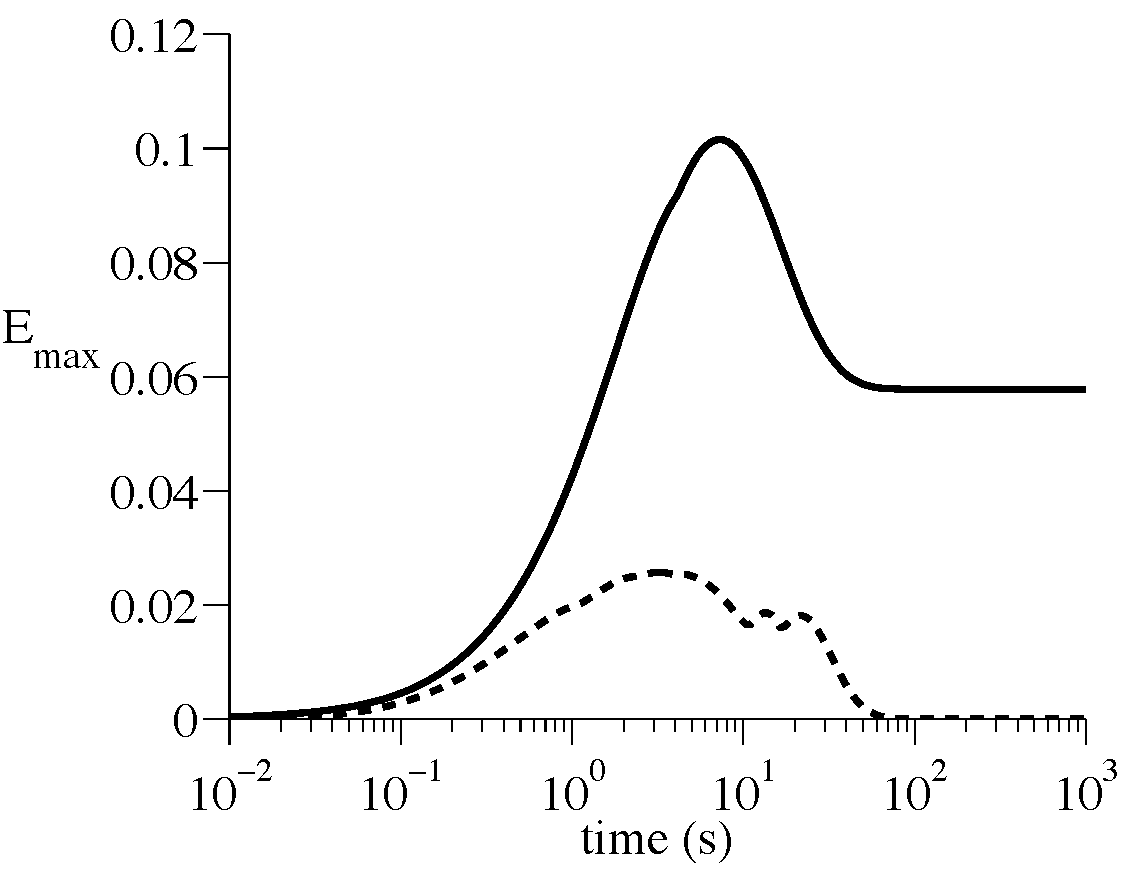
\includegraphics[height=5.8in]{pics/NCDGoldStandard2}
\label{fig:models}
\end{wrapfigure}
\large When the time scales in the \Ca\ release site model are not well separated, the fast/slow reduction error increases because the estimates of the conditional probability distribution within 
blocks ($\hat{\bpi}_i$) become less accurate. 
However, when the rate constants $\hat{q}_{ij}$ of the reduced model are calculated using the
exact conditional probability distribution  $\bar{\bpi}_i$,
\bne \nonumber\hat{q}_{ij} = \bar{\bpi}_i \bQ_{ij} \be_j \ \mbox{for} \ i\neq j,
\ene
both the transient and  limiting ($t\rightarrow \infty$) reduction errors improve (dashed line).
Note that the storage required to calculate the exact conditional distributions is 
far in excess of that needed to estimate them via fast/slow approximation. To overcome this problem, we employ iterative aggregation/disaggregation (IAD) methods [1] to calculate the stationary distribution of full \Ca\ release site models. {\bf Numerical experiments benchmarking automated reductions of release sites composed of up to 80 RyRs consistently yielded small residuals.}
\end{textblock}


\begin{textblock}{7.5}(15.75,4.9)
\Head{--- Model Reduction with No Time Scale Separation ---}
\begin{wrapfigure}{l}{8.0in}
\vspace{-0.1in}
\includegraphics*[height=6in]{pics/GAresult}
\end{wrapfigure}
\large When time scale separation is absent from the full model, a {\bf genetic algorithm is applied to search all possible partitions for those that result in low-error reduced models whose size is arbitrarily decided by the user.}  If a $\hat{\beta}$-state reduced model is required, 
the program will search partitions that divide the full model into $\hat{\beta}$ groups for those that yield low-error reductions (red).  A small `population' of partitions is randomly selected and the `fitness' of each partition is evaluated (blue).  The next generation of partitions is constructed as mutants of current generation partitions randomly sampled in a manner that favors high fitness (i.e., small reduction error).  

\begin{wrapfigure}{r}{7.0in}
\includegraphics*[height=7.0in, angle=270]{pics/GAerror}
\end{wrapfigure}
The genetic algorithm-based reduction method can be extended to compositionally defined \Ca\ release sites with more realistic coupling. For example, when depletion of SR \Ca\ is represented and the diadic subspace [\Ca] is given by
\vspace{-0.05in}
\[
\ca(t) = c_\infty + f\( N_O, c_{SR} \),
\vspace{-0.05in}
\]
the method yields reduced models with their errors $<$1$\%$ for a wide range of SR [\Ca] ($C_{SR}$, right).
\end{textblock}

\begin{textblock}{7.5}(15.75,11.0)
%\hrule\medskip
\Head{--- References ---}
\vspace{-0.3in}
\begin{description}
\item{[1]} \ W. Stewart, \textit{Introduction to the numerical solution of Markov chains}, Princeton Univ.~Press (1994).
\item{[2]} \ J. Keizer and L. Levine. Ryanodine receptor adaptation and \Ca-induced \Ca\ release-dependent \Ca\ oscillations, {\it Biophys J} 71(6):3477 (1996). 
\item{[3]} \ Y. Hao, P. Kemper and G. D. Smith.  Reduction of calcium release site models via fast/slow analysis and iterative 
aggregation/disaggregation, {\it Chaos} 19:037107 (2009).
%\item{[4]} H. DeRemigio, P. Kemper, M. D. LaMar, and G. D. Smith, \textit{Markov chain models of coupled intracellular calcium channels: Kronecker structured representations and benchmark stationary distribution calculations}, Pacific Symposium on Biocomputing (2008), pp. 354--365.
\end{description}

%\medskip\hrule
\end{textblock}

\begin{textblock}{23}(0, 12.25)
%\hrule\medskip
\begin{center}
\color{DarkBlue}
%This material is based upon work supported by the National Science Foundation under Grants 0133132 and 0443843.
\end{center}
%\medskip\hrule
\end{textblock}

\begin{textblock}{23}(8.8,12.3)
Supported by the National Science Foundation under Grant No.~0443843
%\begin{figure}
%
\includegraphics[height=1.5in]{pics/NSFlogo}
%\end{figure}
\end{textblock}

\begin{textblock}{1}(7.8,12)
\begin{figure}

\includegraphics[height=1.5in]{pics/NSFlogo}
\end{figure}
\end{textblock}

\begin{textblock}{1}(14.6,12)
\begin{figure}

\includegraphics[height=1.5in]{pics/NSFlogo}
\end{figure}
\end{textblock}

\end{document}
